\documentclass[a4paper,12pt]{article}
%\documentclass[a4paper,12pt]{article}
\usepackage{comment}
\usepackage{lipsum}
% \usepackage{multirow}
\usepackage{subcaption}
\usepackage{hyperref}
\usepackage{xcolor}
\usepackage{amsmath}
\usepackage{wrapfig}    % inline figures
\usepackage{enumitem}
% \usepackage{mwe}
\usepackage{graphicx} % Use for Images
\usepackage{here}     % Forced Figure Placement
\usepackage{pslatex}	% Use PostScript Fonts
\usepackage{fancyhdr} % Use headers
\usepackage{float}
% Here I keep the left and right margins equal. You can choose to have unequal margins if you want a two-sided book effect.
\usepackage[
	top    = 1.5cm,
	bottom = 1.80cm,
	left   = 2.00cm,
	right  = 2.00cm,
	includeheadfoot]{geometry} % Use similar margins to the Word Template
\setlength{\parindent}{0pt}



% Define the page styles
\fancypagestyle{titlepage}{
	\fancyhf{}
	\fancyhead[C]{
\includegraphics[width=\textwidth]{images/banner.png}}
	\renewcommand{\headrulewidth}{1pt}
}

%\fancypagestyle{body}{
%	\fancyhf{}
%  \fancyhead[C]{
\includegraphics{images/banner.png}}
%}

\fancypagestyle{body}{
    \fancyhf{}
    \fancyhead[C]{
\includegraphics[width=.8\textwidth]{images/banner.png}}
    % \setlength{\headsep}{1pt}
    % \addtolength{\topmargin}{-45.11401pt}
    % \setlength{\headheight}{77.11401pt}
    % \fancyhead[LE,RO]{\thepage}
    \renewcommand{\headrulewidth}{.8pt}

    % \fancyhead[RE,LO]{Chapter \leftmark}
    
}

\fancypagestyle{contents}{
    \fancyhf{}
    \fancyhead[LE,RO]{\thepage}
    \fancyhead[RE,LO]{\leftmark}
}

\fancypagestyle{appendix}{
    \fancyhf{}
    \fancyhead[LE,RO]{\thepage}
    \fancyhead[RE,LO]{APPENDICES}
}

\fancypagestyle{acknowledgements}{
    \fancyhf{}
    \fancyhead[LE,RO]{\thepage}
}


\renewcommand{\headrulewidth}{1.5pt}
\renewcommand{\arraystretch}{1.2}
\usepackage{tabularx}

% include bibliography in table of contents
%\usepackage[nottoc,numbib]{tocbibind}
\usepackage[nottoc]{tocbibind}
\renewcommand{\refname}{References}

% Stylistic note: I use `\\` at the end of every paragraph to give some space between two paragraphs because I think it looks neater. You can change the inter-paragraph spacing by using 
% \setlength{\parskip}{1em} [Note that this may affect how the lines in the content pages are spaced]
% instead of `\\` at the end of each paragraph
% or you can leave it out altogether if you want no spacing between paragraphs

% Begin the actual document
\begin{document}
\pagestyle{body}

%\setlength{\headheight}{50pt}

\title{
    \vspace{1cm}
        {\bf
        {\Huge Proxy Attention : Comparing and Combining Augmentation with Attention\\
        % \vspace{2mm}Som\\
        }
        }
        \vspace{4mm}Graduation Project Proposal\\(Computational Intelligence and Robotics)\\
        \vspace{4mm}Subhaditya Mukherjee (s4747925)\\Oct 25 2022\\
        \vspace{10cm}{\LARGE Internal Supervisor(s): S.H. Mohades Kasaei, PhD (Artificial Intelligence, University of Groningen)}\\
        {\bf {Artificial Intelligence\\University of Groningen, The Netherlands}}
}
\date{}

\maketitle
\thispagestyle{titlepage}


% \newpage

% \thispagestyle{titlepage}

% \vspace*{4cm}

% \begin{center}
%     {\bf{\large University of Groningen}}\\
%     \vspace{1cm}{\bf{\large Credit Assignment for Surrogate Gradient\\\vspace{1mm}Learning Rules in Spiking Neural Networks}}\\
%     \vspace{2cm}{\bf Master's Thesis}\\
%     \vspace{0.5cm}To fulfill the requirements for the degree of\\Master of Science in Artificial Intelligence\\
%     at University of Groningen under the supervision of\\
%     Prof. dr. L.R.B. Schomaker (Artificial Intelligence, University of Groningen)\\
%     and\\
%     Prof. dr. Tamalika Banerjee (Zernike Institute for Advanced Materials, University of Groningen)\\
%     \vspace{3cm}{\bf Manvi Agarwal (s1234567)}\\
%     \vspace{4cm}\today
    
% \end{center}

\newpage

\setlength{\headheight}{32pt}

% \thispagestyle{acknowledgements}    % remove this if you want `CONTENTS' to appear in the header of the first Contents page
% \pagestyle{contents}

%\setlength{\headheight}{32pt}

\tableofcontents
\addtocontents{toc}{~\hfill\textbf{Page}\par}

% incase the contents spill onto another page use this for help: https://tex.stackexchange.com/questions/8296/add-page-above-page-numbers-in-table-of-contents

% \include{chapters/acknowledgements}
\thispagestyle{body}
\section{Introduction}
Over the past decade or so, Computer Vision (CV) has taken over the world. Almost every domain, ranging from medicine to robotics has been affected in some way or the other because of it. At the heart of all of these improvements, reside Neural Network architectures. There are thousands of architectures, each made to serve a different purpose, some vastly better than the other. But for each of them, there exists tradeoffs. Accuracy, Memory, Time to train, Cost to run etc. Scaling up these models requires a massive amount of energy, with some consuming upwards of 27,648 kilowatt hours of electricity just to train. This is around the same amount that three households use in a whole year. \href{https://www.techtarget.com/searchenterpriseai/feature/Energy-consumption-of-AI-poses-environmental-problems}{source}. And this is just one model.\\
In order to get any kind of prediction from them, these networks need to be fed large quantities of data. This training consumes a vast amount of resources that becomes increasingly harder to provide in niche problems where only a small amount of data is available. Models that outperform existing benchmarks such as the Swin Transformer \cite{liu_swin_2022} require an abysmal amount of data and energy. This makes it extremely hard for smaller companies, research labs and individuals to use this technology.\\
The second major flaw of these systems is due to the extremely complex, high dimensional manifolds they try to model. Because of such high dimensionality, it becomes next to impossible to predict exactly why a network made the decision it did. This becomes extremely important in situations like performing medical diagnoses. Not knowing why a network said what it did, makes it very hard to trust. The rise of Explainable AI (XAI) attempts to solve this issue.\\
In order to tackle the lack of data, many methods such as transforming the present data in multiple ways to increase the available data points aka data augmentation have been created. Methods like transfer learning enable using pre-trained networks to "fine-tune" on a specific dataset. In the traditional sense, the fields of XAI and data augmentation are not related. So far, the outputs of XAI algorithms have just been used as an explainibility measure, not for training.
Therefore, combining these concepts, we arrive at a novel Augmentation technique that uses Saliency maps as an input during training to emulate Attention \cite{vaswani_attention_2017} mechanisms. We call this "Proxy Attention".\\
The objective of this thesis is to design a novel informed augmentation method that would not only reduce the requirement of data, but will also be more memory and time efficient during training as compared to current algorithms in turn building on the advances of XAI to improve training performance.
\thispagestyle{body}

\section{Theoretical Framework} \label{section:thero}
The literature that this thesis builds upon is explained below. 
\subsection*{Explainibility}
% Gradcam etc
It is commonly noted that neural networks are black boxes. Although in the past decade, these NNs have performed vastly better than a lot of computer vision algorithms, their results are still hard to explain. Due to the high dimensionality of the feature space representation that they create, it becomes impossible to directly visualize the reasons for the decisions made by these networks. The field of Explainable AI (XAI) rose to deal with these challenges. One of the most notable algorithms in this domain for image classification is that of CAM \cite{oquab_is_2015} (eventually succeeded by Grad-CAM \cite{selvaraju_grad-cam_nodate} and then by Grad-CAM++ \cite{chattopadhyay_grad-cam_2018}). The main idea is to visualize the gradients of the final convolutional layer in a trained network to create a sort of "activation map". This map could essentially be used to visualize which parts of the image the network used to make its decision.\\
In CAM \cite{oquab_is_2015}, the final layer would have to be replaced by a Global Average Pooling \cite{lin_network_2014} followed by a Softmax. This would then require retraining the network. Since this was not very feasible, further research came up with Grad-CAM \cite{selvaraju_grad-cam_nodate}. In this paper, the authors proposed using backpropagation over the image and using class information to create the attention map. This makes it able to be directly applied to any network meant for vision classification. The drawback of this method though, was that it sometimes failed when there was more than one instance of the object in the image. It also sometimes failed to fully cover the object in the attention map. Grad-CAM++ \cite{chattopadhyay_grad-cam_2018} solves this issue by modifying the backpropagation algorithm which now scales the map by considering the size of the response.\\
In this thesis, we want to examine using images weighted by the outputs of Grad-CAM and Grad-CAM++ as augmentation methods during training. 
\subsection*{Augmentation}
% Random Erasing, Saliency Mix
It is not always possible to have a huge amount of data when it comes to training a network. To maximize the performance that can be achieved with existing data, performing transformations to the images either before or during training has become a norm. This is called Augmentation and in a lot of cases, it helps in improving the performance \cite{perez2017effectiveness}. There are numerous variants of this, ranging from flipping the image on either axis, random cropping, randomly erasing parts of the image, isolating color channels, etc. In this paper, we build on two such techniques.\\
Random Erasing \cite{zhong2020random} is an algorithm in a random region from which the image is deleted. The region size is randomly defined at every instance of running the algorithm. Combined with other such Augmentation, this improves performance by a significant amount. The second algorithm is called Visual Context Augmentation \cite{dvornik2018modeling} in which a network for object detection learns about context by being given data where the object to be detected is blacked out and other images are around it. Many such images with different contexts for the same object are generated and then the network is trained. This teaches the network to predict the object in time.\\
In this thesis, we combine Augmentation and Explainability to create the proposed "Proxy Attention".
\subsection*{Attention}
One of the challenges with any neural network is deciding what parts of an image or a sentence are important for the final decision.
In Natural Language Processing, Sequence2Sequence models (eg: RNN, LSTM, etc) had been used for a long time, but they had the critical flaw of not being able to work over very long sentences. In time, Vaswani et al. \cite{vaswani_attention_2017}, in their seminal paper "Attention Is All You Need", proposed a type of attention called Scaled Dot Product Attention as part of a new architecture they titled the "Transformer". This modification allowed the network to not only learn how to classify but also learn which parts are important. Transformer based models such as BERT \cite{devlin_bert_2019} and GPT-3 \cite{brown_language_2020} then suddenly overtook RNNs, LSTMs etc.
\subsection*{ViT}
% Good/Bad/Moderates
The Transformer used to be generally only used in NLP, but recently \cite{dosovitskiy2020image} converted the Transformer pipeline to work with Images, and the Vision Transformer (ViT) was created. This of course led to a boom in using Transformers for Vision but these networks require even more massive amounts of data compared to CNNs. Transfer learning alleviates this issue to an extent, but not fully. This is a huge problem.

To examine the effects of Proxy Attention, we compare results to the ViT as well. The aim is to combine them both if this combination ends up being significant.
\thispagestyle{body}
\section{Research Questions} \label{section:researchq}
The main research questions that summarize the aims of this study are as follows.
\begin{itemize}
    \item Is it possible to create an augmentation technique based on Attention maps?
    \item Is it possible to approximate the effects of Attention from ViTs in a CNN?
    \item Is it possible to make a network converge faster using the outputs from XAI techniques?
\end{itemize}
\thispagestyle{body}
\section{Methods} \label{section:methods}

\subsection{Proposed Pipeline}
To address the posed research questions, the following pipeline is proposed. Note that these stages might be modified later on as the project progresses and new needs are identified. The objective of reducing memory usage and training time remain the same regardless of the change.

\subsubsection*{Stage 0 - Setup}
Since there are a lot of experiments to be run, a configuration file is created with all the parameters required per network and data. Every dataset has it's own path, definition of labels, and image sizes. To ensure compatibility with future research, this type of configuration is very important. Specific Dataloaders for each configuration will have to be created.
To ensure proper comparision, the images will all be resized to a common size of 224x224. 

\subsubsection*{Stage 1 - Intial Training}
The first stage of the main pipeline is pre-training. This will be done by fine tuning the model on the chosen dataset by transfer learning from a pretrained ImageNet model, if it exists for the chosen model. The number of epochs to train here is yet to be decided. Once this initial training is done, the model is saved for the next stage and the memory is cleared to prevent the GPU from being overloaded.
While training, the gradients for the final layer could be saved using Pytorch Hooks which is just a means to "hook" into the training pipeline and insert arbitrary computation steps.

\subsubsection*{Stage 2 - Proxy Attention}
The Proxy Attention stage involves first identifying the images that the model incorrectly classified from the training data. Note that this is not an inference step, but an intermediate, therefore validation data is not used now. After these images are identified, the activations of the final layer wrt each of these images is computed and reshaped into a "map" with the same size of the image. The highest values of this activation map are thresholded, and these locations are mapped back onto the original image. In the original image, these areas of high activations are replaced with a black pixel. These images are then saved to the disk.

\subsubsection*{Stage 3 - Retraining}
Stage 1 is repeated with the new data along with the original images. Until a satsifactory performance is achieved, this loops back to Stage 1.

\subsection{Frameworks}
The existing frameworks that will be used to speed up this research effort are as follows: 
\begin{itemize}
\item Pytorch\cite{paszke2019pytorch}: For the entire deep learning backbone
\item OpenCV\cite{bradski2000opencv}: For optimized reading of images
\item Fastai\cite{howard2018fastai}: A wrapper on Pytorch that enables faster experimentation 
\end{itemize}

\subsection{Dataset and Models}
The Datasets and Models to be used are yet to be decided. But in general, the evaluation will start with simpler datasets like the \href{https://www.kaggle.com/datasets/grassknoted/asl-alphabet}{American Sign Language dataset} and move onto more complex ones.
The same applies to the models. Intial experiments will start with ResNet \cite{he2016deep} and move on to more complex models. Eventually the ViT \cite{dosovitskiy2020image} will also be used.

\subsection{Evaluation}
Evaluation is one of the most important steps to the pipeline in this project. The following metrics are considered now, but research needs to be done on which to include and other metrics to be added.
\begin{itemize}
    \item The Accuracy, Precision and Recall of the predictions on the validation set
    \item The time taken to train as compared to the same network without Proxy Attention
    \item Comparision with ViT \cite{dosovitskiy2020image} and the presence/abscence of Attention
    \item The amount of GPU RAM used for training
\end{itemize}
These metrics have to be added into the pipeline to avoid having to manually compute them.

\subsection{Tackling Potential Issues}
Since this is still an experimental procedure, some issues come to mind. This section aims to provide some answers to them. It is to be noted that further issues may rise during implementation, but these are not known as of now and will be brought to light in time.
\subsubsection*{Memory Constraints}
To reduce memory usage we use the following measures.
\begin{enumerate}
    \item Unloading the model and it's weights after every stage so it stops using the GPU RAM.
    \item Saving the augmented images to the disk instead of keeping them in memory.
    \item Using Mixed Precision Training whereby most of the computation is performed in 16bit floats instead of the usual 32bits.
    \item Using transfer learning throughout the process.
\end{enumerate}
\subsubsection*{Computation Time for Activations}
Computing the activations can be costly, so some measures will be taken to overcome them.
\begin{enumerate}
    \item Attempt to parallelize the final prediction over all the images in a batch.
    \item Use Pytorch hooks to pre compute these activations as in part they would be computed during training.
\end{enumerate}
\subsubsection*{Accuracy vs Confidence}
While attempting to flesh out this idea, I realized that that it would be interesting to utilize the confidence of predictions along with the accuracy in order to see if this made any difference. This will possibly be discussed in the future.

\thispagestyle{body}
\section{Scientific Relevance for Artificial Intelligence} \label{section:relevance}
Training networks on new data is a fundamental task in AI. But for a majority of researchers and startups, the cost of this training is quite high. Also considering the lack of large amounts of data for specific use cases, a need to reduce the training time and require less data during training is ever present.\\
This research focuses on performing a more informed augmentation that hopes to reduce these problems and allow for faster training with lesser data. In the process, it attempts to use advances in field of XAI to improve training. Further, this project leads into the field of continual learning where adding new information is quite costly and presents a method to reduce this cost.\\
More specifically, this project aims to make the following contributions to the literature:
\begin{itemize}
    \item Create a new informed Augmentation method that uses saliency outputs as a sort of Proxy-Attention to improve performance
    \item Use advances in the field of XAI to empower networks directly
    \item Contrast using a ViT \cite{dosovitskiy2020image} with a Convnet + Proxy Attention
    \item Reduce training cost and time of networks so as to aid in continual learning
\end{itemize}
\thispagestyle{body}
\section{Planning} \label{section:plan}
The following plan contains the work parts (WP) of this graduation thesis and the expected breakdown of how long it would take to work on each of them. There are eight such WPs distributed over 32 weeks as follows : 
\begin{itemize}
    \item WP1	Literature study of gradient based XAI algorithms and overview of project
    \item WP2	Identifying datasets, metrics, optimizations required to build the pipeline
    \item WP3	Implementing the base framework, dataset loaders, metrics and optimisations
    \item WP4	Implementing the gradient based algorithms, Integrating Vision Transformers into the pipeline
    \item WP5	Perform Training, Experimentation with different modules, Hyper Parameter Optimization
    \item WP6	Testing and analysis
    \item WP7	Writing the report
    \item WP8	Preparing final presentation
\end{itemize}
\begin{figure}[!htbp]
  \centering
  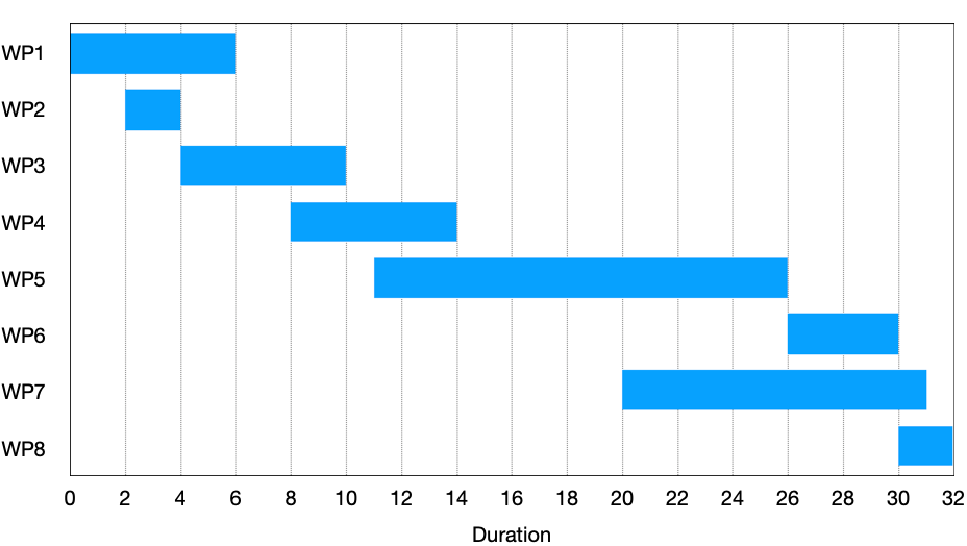
\includegraphics[width=.8\textwidth]{images/gantt_chart.pdf}
  \caption{Weekly Plan}
  \label{fig:plan}
\end{figure}

The timeline of the research is presented in this \hyperref[fig:plan]{Figure \ref{fig:plan}}.

\section{Resources and Support}
For the initial creation, testing and ideation of pipelines and network architecture,Wewill use my personal computer. It runs Linux and has a decent GPU. For the final testing of multiple architectures and models,Wewill make use of the Peregrine HPC Cluster's virtual NVIDIA Tesla v-100 nodes soWecan run batch experiments.\\
This work will be directly supervised by Dr. Hamidreza Kasaei. A co-supervisor is yet to be determined. The plan for meetings is to have a progress update every two weeks until completion. This schedule should remain stable for most of the project. There is no collaboration with any company so other related points do not apply here.
\pagestyle{body}

\bibliographystyle{ieeetr}
\bibliography{biblio}

% \chapter{Appendix}
\subsection{Summary of Results Per Dataset}
This section shows the accuracies per model for each dataset. The results are shown in Table ~\ref{tab:summary_ds}.
\begin{table}[H]
\centering
\resizebox{0.8\columnwidth}{!}{%
\begin{tabular}{lllr}
\toprule
         &                      &          &   accuracy \\
ds\_name & model & step\_schedule &            \\
\midrule
dogs & efficientnet\_b0 & Proxy &  94.630158 \\
         &                      & No Proxy &  85.605498 \\
cifar100 & vit\_base\_patch16\_224 & Proxy &  75.651538 \\
         &                      & No Proxy &  54.910000 \\
\bottomrule
\end{tabular}
}
\caption{Summary of results on different datasets}
\label{tab:summary_ds}
\end{table}

\end{document}